\section{Hash-and-Resubmit variations}
\label{sec:hash-appendix}
% Now consider a variation of the above game, in
% which $\pla$ calls \texttt{\proc$_1$(}$\arra$\texttt{)}, and then calls
% \texttt{pickSpan(}$m, n$\texttt{)} that determines the span of $\arra$ which
% can be contested. In reality, $\plb$ only needs to re-send $\arras[m:n]$ in
% order to perform the comparison $\arra[m:n] < \arrb$. However, the digest of
% $\arra$ is calculated by hashing the entire structure. Therefore, the
% $resubmit$ phase cannot be successfully performed by rehashing $\arras[m:n]$,
% because \texttt{H(}$\arra$\texttt{)} $\ne$ \texttt{H(}$\arra[m:n]$\texttt{)}.
In order to enable selective dispatch of a segment of interest, different
hashing schemas can be adopted, such as Merkle Trees ~\cite{merkle} and Merkle Mountain
Ranges ~\cite{mmr-1,mmr-2}. In this variation of the pattern, which we term
\emph{merkle-hash-and-resubmit}, the commitment of an array $\data$ is
a Merkle Tree Root (MTR). In the \emph{resubmit} phase, $\data[m{:}n]$ is
dispatched, accompanied by the siblings that reconstruct the MTR of
$\data$.

\begin{figure}[h]
    \vspace*{-5mm}
    \begin{center}
        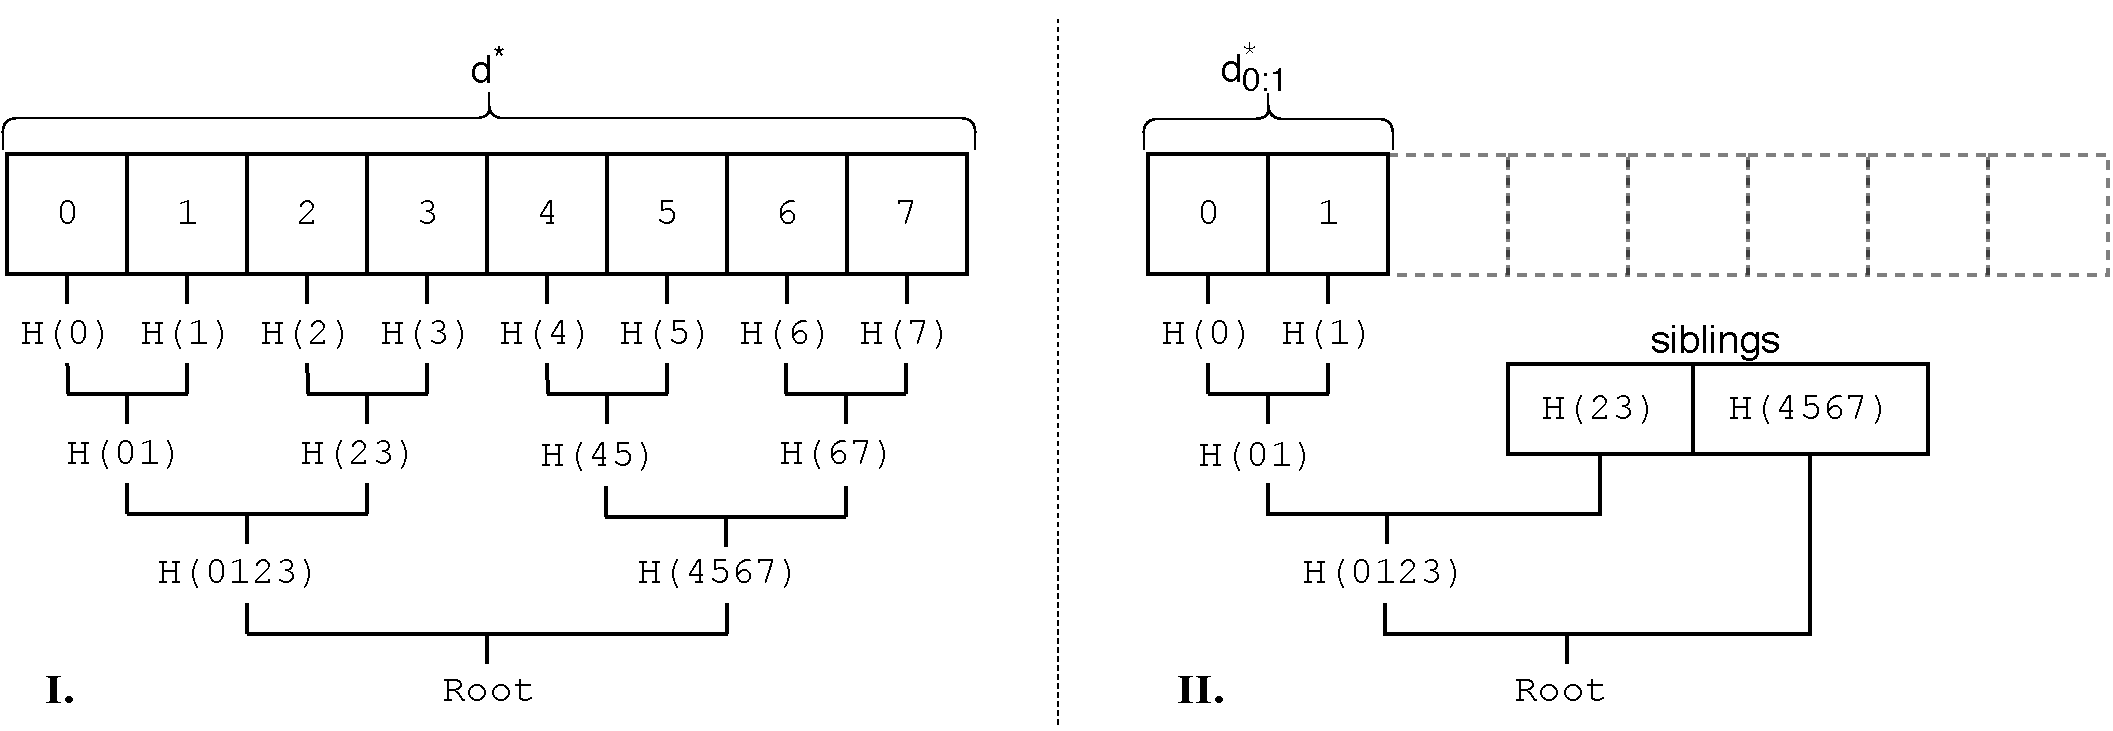
\includegraphics[width=0.8\linewidth]{figures/merkle-har.pdf}
    \end{center}
    \vspace*{-5mm}
    \caption{\textbf{I.} The calculation of root in \emph{hash} phase.
    \textbf{II.} The verification of the root in \emph{resubmit} phase.
    \textsf{H}($k$) denotes the digest of element $k$. \textsf{H}($kl$) denotes the
    result of \textsf{H}(\textsf{H}($k$) $|$ \textsf{H}($l$))}
    \label{fig:merkle-har}
    \vspace*{-4mm}
\end{figure}

This variation of the pattern removes the burden of sending redundant data,
however it implies on-chain construction and validation of the Merkle
construction. In order to construct a MTR for an array $\data$,
$|\data|$ hashes are needed for the leafs of the MT, and $|\data| -
1$ hashes are needed for the intermediate nodes. For the verification, the
segment of interest $\data[m{:}n]$ and the siblings of the MT are hashed.
The size of siblings is approximately $log_2(|\data|)$. The process of
constructing and verifying the MTR is displayed in Figure
~\ref{fig:merkle-har}.

In Solidity, different hashing operations vary in cost. An invocation of
\textsf{sha256}($\data$), copies $\data$ in memory, and then the
\emph{CALL} instruction is performed by the EVM that calls a pre-compiled
contract. At the current state of the EVM, \emph{CALL} costs 700 gas units, and
the gas paid for every word when expanding memory is 3 gas units~\cite{wood}.
Consequently, the expression $1 \times \textsf{sha256}(\data)$ costs less than
$|\data| \times $\textsf{sha256}(1) operations. A different cost policy applies
for \textsf{keccak}~\cite{keccak} hash function, where hashing costs 30 gas
units plus 6 additional gas far each word for input data~\cite{wood}. The usage
of \textsf{keccak} dramatically increases the performance in comparison with
\textsf{sha256}, and performs better than plain rehashing if the product of
on-chain processing is sufficiently larger than the originally dispatched data.
Costs of all related operations are listed in Table~\ref{tab:operations-gas}.

The merkle variation can be potentially improved by dividing $\data$ in
chunks larger than 1 element. We leave this analysis for future work.

\begin{figure}[H]
    \vspace*{-5mm}
    \begin{center}
        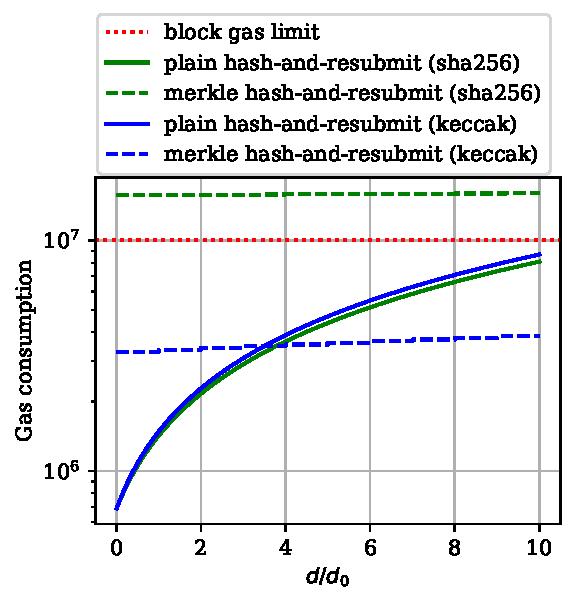
\includegraphics[width=0.9\columnwidth]{figures/har-vs-mhar.pdf}
    \end{center}
    \vspace*{-7mm}
    \caption{Trade-offs between \emph{hash-and-resubmit} variations. In the
    vertical axis the gas consumption is displayed. In the horizontal axis the
    size of $\data$. The size of $d_0$ is 10KB bytes, and the hash functions we
    use are the pre-compiled \texttt{sha256} and \texttt{keccak}.}
    \label{fig:har-vs-mhar}
    \vspace*{-4mm}
\end{figure}

In Table~\ref{tab:har-vs-mhar} we display the operations needed for hashing and
verifying the underlying data for both variations of the pattern as a function
of data size. In Figure~\ref{fig:har-vs-mhar} we demonstrate the gas
consumption for dispatched data of 10KB, and varying size of on-chain
process product.

\begin{table}[!h]
\begin{tabular}{|c|c|}
\hline
\textbf{Operation} & \textbf{Gas cost} \\ \hline
\textsf{load}($\data$)            & $ \data_{bytes} \times 68 $          \\ \hline
\textsf{sha256}($\data$)          & $\data_{words} \times 3 + 700 $     \\ \hline
\textsf{keccak}($\data$)          & $\data_{words} \times 6 + 30 $      \\ \hline
\end{tabular}
\caption{Gas cost of EVM operations as of June 2020.}
\label{tab:operations-gas}
\vspace*{-5mm}
\end{table}

\newcommand{\mydata}{\data}

\begin{table}[h]
\begin{tabular}{|c|c|c|}
\hline
\textbf{\begin{tabular}[c]{@{}c@{}}phase per\\variance\end{tabular}} &
\textbf{\begin{tabular}[c]{@{}c@{}}plain hash\\and resubmit\end{tabular}} &
\textbf{\begin{tabular}[c]{@{}c@{}}merkle hash\\ and resubmit\end{tabular}} \\ \hline
\textbf{hash} &
\textsf{H}($\mydata$) &
\begin{tabular}[c]{@{}c@{}}
    \textsf{H}($\mydata_{elem}$) $\times\ |\mydata|$ \\ \textsf{H}(digest)
$\times\ (|\mydata|-1)$

\end{tabular} \\ \hline
\textbf{resubmit} &
\textsf{load}($\mydata$) + \textsf{H}($\mydata$) &
\begin{tabular}[c]{@{}c@{}}
    \textsf{load}($\mydata[m{:}n])$ + \\
    \textsf{load}($siblings$) + \\
    \textsf{H}($\mydata[m{:}n])$ + \\
    \textsf{H}($digest$)$\times |siblings|$
\end{tabular} \\ \hline
\end{tabular}

\caption{Summary of operations for \emph{hash-and-resubmit} pattern variations.
$\mydata$ is the product of on-chain operations and $\mydata_{elem}$ is an
element of $\mydata$. \textsf{H} is a hash function, such as \textsf{sha256}
or \textsf{keccak}, $digest$ is the product of \textsf{H}(.) and $siblings$ are
the siblings of the Merkle Tree constructed for $\mydata$.
}

\label{tab:har-vs-mhar}
\vspace*{-10mm}
\end{table}

